\documentclass[tikz,border=8pt]{standalone}
\usepackage{amsmath,amssymb}
\usetikzlibrary{arrows.meta,calc,decorations.markings,decorations.pathmorphing,patterns,shapes.geometric,positioning}

\begin{document}
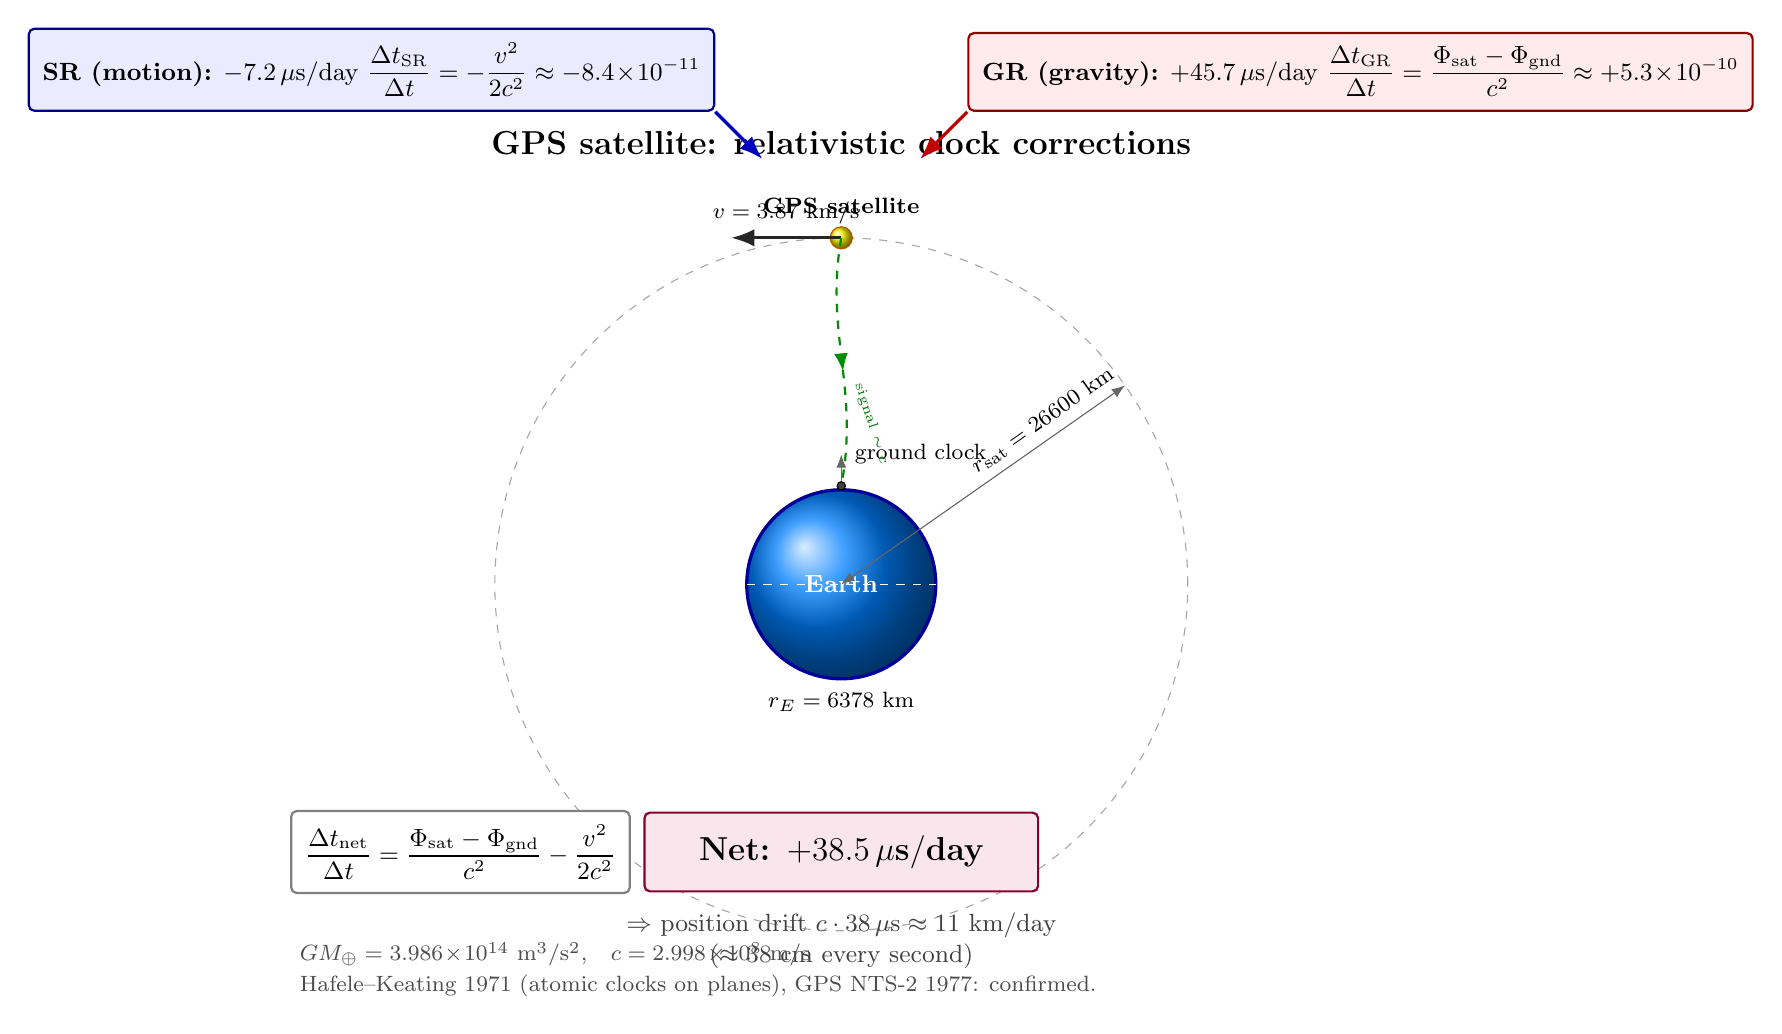
\begin{tikzpicture}[>=Latex,
  earthball/.style={ball color=blue!50!cyan, draw=blue!60!black, very thick},
  satdot/.style={circle, ball color=yellow!90!orange, draw=orange!70!black, thin, inner sep=0pt, minimum size=8pt},
  obsperson/.style={circle, fill=black!75, draw=black, thin, inner sep=0pt, minimum size=3pt},
  signalpath/.style={draw=green!55!black, thick, dashed, decoration={markings, mark=at position 0.55 with {\arrow{>}}}, postaction={decorate}},
  srarrow/.style={->, very thick, blue!75!black},
  grarrow/.style={->, very thick, red!75!black},
  netarrow/.style={->, ultra thick, purple!80!black},
  formulabox/.style={draw=black!50, thick, rounded corners=2pt, fill=yellow!8, inner sep=5pt, font=\small}]

  % --- Title ----------------------------------------------------------------
  \node[font=\large\bfseries, anchor=center] at (0, 5.6)
    {GPS satellite: relativistic clock corrections};

  % --- Earth ----------------------------------------------------------------
  \def\REarth{1.2}
  \draw[earthball] (0, 0) circle (\REarth);
  \node[font=\small\bfseries, white] at (0, 0) {Earth};

  % Equator dashed line
  \draw[draw=white!90, thin, dashed] (-\REarth, 0) -- (\REarth, 0);

  % Earth label
  \node[font=\footnotesize, anchor=north] at (0, -\REarth-0.05) {$r_E = 6378$~km};

  % --- Ground observer ------------------------------------------------------
  \node[obsperson] (gnd) at (0, \REarth+0.05) {};
  \draw[->, thin, black!60] (gnd) -- ++(0, 0.4);
  \node[font=\footnotesize, anchor=west] at (0.05, \REarth+0.45) {ground clock};

  % --- Orbit circle ---------------------------------------------------------
  \def\Rorbit{4.4}
  \draw[draw=black!35, thin, dashed] (0, 0) circle (\Rorbit);

  % Orbit radius arrow
  \draw[<->, thin, black!60] (0, 0) -- ($(35:\Rorbit)$);
  \node[font=\footnotesize, anchor=south west, rotate=35] at ($(35:\Rorbit/2.1)$) {$r_{\rm sat}=26600$~km};

  % --- GPS satellite --------------------------------------------------------
  \coordinate (sat) at (90:\Rorbit);
  \node[satdot] (satnode) at (sat) {};
  \node[font=\footnotesize\bfseries, anchor=south] at ($(sat)+(0,0.18)$) {GPS satellite};

  % Velocity vector (tangent to orbit, leftward at top of orbit)
  \draw[->, very thick, black!85] (sat) -- ++(-1.4, 0);
  \node[font=\footnotesize, anchor=south] at ($(sat)+(-0.7, 0.05)$) {$v=3.87$~km/s};

  % --- Signal path ----------------------------------------------------------
  \draw[signalpath] (sat) to[out=-100, in=80] (gnd);
  \node[font=\tiny, text=green!45!black, anchor=west, rotate=-72] at ($(sat)!0.55!(gnd)+(0.18,0)$)
    {signal $\sim c$};

  % --- Two correction arrows around the satellite --------------------------
  % SR slow arrow (blue), to the upper-left, away from satellite
  \begin{scope}[shift={($(sat)+(-1.6, 1.6)$)}]
    \node[formulabox, anchor=south east, fill=blue!8, draw=blue!55!black] (srbox) at (0,0)
      {\textbf{SR (motion):} $-7.2\,\mu\text{s}/\text{day}$\\[1pt]
       $\dfrac{\Delta t_{\rm SR}}{\Delta t}=-\dfrac{v^2}{2c^2}\approx-8.4\!\times\!10^{-11}$};
    \draw[srarrow] (srbox.south east) -- ++(0.6, -0.6);
  \end{scope}

  % GR fast arrow (red), to the upper-right, toward satellite
  \begin{scope}[shift={($(sat)+(1.6, 1.6)$)}]
    \node[formulabox, anchor=south west, fill=red!8, draw=red!55!black] (grbox) at (0,0)
      {\textbf{GR (gravity):} $+45.7\,\mu\text{s}/\text{day}$\\[1pt]
       $\dfrac{\Delta t_{\rm GR}}{\Delta t}=\dfrac{\Phi_{\rm sat}-\Phi_{\rm gnd}}{c^2}\approx +5.3\!\times\!10^{-10}$};
    \draw[grarrow] (grbox.south west) -- ++(-0.6, -0.6);
  \end{scope}

  % --- Net correction big label --------------------------------------------
  \node[formulabox, anchor=center, fill=purple!10, draw=purple!70!black, font=\large\bfseries,
        minimum width=5cm, minimum height=1cm]
    at (0, -3.4)
    {Net: $+38.5\,\mu\text{s}/\text{day}$};

  % Sub-label below: drift if uncorrected
  \node[font=\small, anchor=north, text=black!75, align=center]
    at (0, -4.05)
    {$\Rightarrow$ position drift $c\cdot 38\,\mu\text{s}\approx 11$~km/day\\
     ($\approx 38$~cm every second)};

  % --- Legend / addition formula -------------------------------------------
  \node[formulabox, anchor=west, fill=white]
    at (-7.0, -3.4)
    {$\dfrac{\Delta t_{\rm net}}{\Delta t}=\dfrac{\Phi_{\rm sat}-\Phi_{\rm gnd}}{c^2}-\dfrac{v^2}{2c^2}$};

  % Footer / data row
  \node[font=\footnotesize, text=black!70, anchor=west]
    at (-7.0, -4.7)
    {$GM_\oplus=3.986\!\times\!10^{14}$~m$^3$/s$^2$,~~ $c=2.998\!\times\!10^8$~m/s};
  \node[font=\footnotesize, text=black!70, anchor=west]
    at (-7.0, -5.1)
    {Hafele--Keating 1971 (atomic clocks on planes), GPS NTS-2 1977: confirmed.};

\end{tikzpicture}
\end{document}
